\documentclass{beamer}
\mode<presentation>
\usepackage{amsmath}
\usepackage{amssymb}
%\usepackage{advdate}
\usepackage{adjustbox}
\usepackage{subcaption}
\usepackage{enumitem}
\usepackage{multicol}
\usepackage{mathtools}
\usepackage{listings}
\usepackage{url}
\def\UrlBreaks{\do\/\do-}
\usetheme{metropolis}
%\usecolortheme{lily}
\setbeamertemplate{footline}
{
	\leavevmode%
	\hbox{%
		\begin{beamercolorbox}[wd=\paperwidth,ht=2.25ex,dp=1ex,right]{author in head/foot}%
			\insertframenumber{} / \inserttotalframenumber\hspace*{2ex} 
		\end{beamercolorbox}}%
		\vskip0pt%
	}
	\setbeamertemplate{navigation symbols}{}

	\providecommand{\nCr}[2]{\,^{#1}C_{#2}} % nCr
	\providecommand{\nPr}[2]{\,^{#1}P_{#2}} % nPr
	\providecommand{\mbf}{\mathbf}
	\providecommand{\pr}[1]{\ensuremath{\Pr\left(#1\right)}}
	\providecommand{\qfunc}[1]{\ensuremath{Q\left(#1\right)}}
	\providecommand{\sbrak}[1]{\ensuremath{{}\left[#1\right]}}
	\providecommand{\lsbrak}[1]{\ensuremath{{}\left[#1\right.}}
	\providecommand{\rsbrak}[1]{\ensuremath{{}\left.#1\right]}}
	\providecommand{\brak}[1]{\ensuremath{\left(#1\right)}}
	\providecommand{\lbrak}[1]{\ensuremath{\left(#1\right.}}
	\providecommand{\rbrak}[1]{\ensuremath{\left.#1\right)}}
	\providecommand{\cbrak}[1]{\ensuremath{\left\{#1\right\}}}
	\providecommand{\lcbrak}[1]{\ensuremath{\left\{#1\right.}}
	\providecommand{\rcbrak}[1]{\ensuremath{\left.#1\right\}}}
	\theoremstyle{remark}
	\newtheorem{rem}{Remark}
	\newcommand{\sgn}{\mathop{\mathrm{sgn}}}
	\providecommand{\abs}[1]{\left\vert#1\right\vert}
	\providecommand{\res}[1]{\Res\displaylimits_{#1}} 
	\providecommand{\norm}[1]{\lVert#1\rVert}
	\providecommand{\mtx}[1]{\mathbf{#1}}
	\providecommand{\mean}[1]{E\left[ #1 \right]}
	\providecommand{\fourier}{\overset{\mathcal{F}}{ \rightleftharpoons}}
	%\providecommand{\hilbert}{\overset{\mathcal{H}}{ \rightleftharpoons}}
	\providecommand{\system}{\overset{\mathcal{H}}{ \longleftrightarrow}}
	%\newcommand{\solution}[2]{\textbf{Solution:}{#1}}
	%\newcommand{\solution}{\noindent \textbf{Solution: }}
	\providecommand{\dec}[2]{\ensuremath{\overset{#1}{\underset{#2}{\gtrless}}}}
	\newcommand{\myvec}[1]{\ensuremath{\begin{pmatrix}#1\end{pmatrix}}}
		\let\vec\mathbf

		\lstset{
			%language=C,
			frame=single, 
			breaklines=true,
			columns=fullflexible
		}

		\numberwithin{equation}{section}

		\title{Matgeo Presentation}
		\author{Arjun Pavanje,\\ EE24BTECH11005,\\IIT Hyderabad.\\}

		\date{\today} 
		\begin{document}

		\begin{frame}
			\titlepage
		\end{frame}

		\section*{Table of Contents}
		\begin{frame}
			\tableofcontents
		\end{frame}
		\section{Problem}
		\begin{frame}
			\frametitle{Problem Statement}

      Solve the differential equation 
\begin{align}
  \brak{y^{\prime \prime \prime}}^2 + \brak{y^{\prime \prime}}^3 + \brak{y^{\prime}}^4 + \brak{y}^5 = 0 
\end{align}
    with initial conditions 
      \begin{align}
        y^{\prime \prime}\brak{x}=0, y^{\prime}\brak{x}=0, y\brak{x}=1
      \end{align}
		\end{frame}
		\section{Solution}
		\subsection{Theoretical Solution}
		\begin{frame}
      \frametitle{Theoretical Solution}
An exact theoretical solution using known methods of solving differential equations was not found; however, it can be approximated to a pretty good degree of precision. Euler's method will be used to obtain a plot of the solution\\		\end{frame}
    \subsection{Computational Solution}
		\begin{frame}
			\frametitle{Computational Solution}
By first principle of derivatives,
      {\small
\begin{align}
    y^{\prime}\brak{t} = \lim_{h\to 0}\frac{y\brak{t+h} - y\brak{t}}{h}\\
    y\brak{t+h} = y\brak{t} + hy^{\prime}\brak{t}
\end{align}
      }

Let $y^{i}$ be the $i^{th}$ derivative of the function, $m$ be the order of the differential equation. Set $y_1=y, y_2=y^{1}, y_3=y^{2} \dots$ so on.\\
We obtain the system,
      {\small
\begin{align}
    \myvec{y_1^{\prime} \\ y_2^{\prime} \\ \vdots \\ y_{m-1}^{\prime} }&=\myvec{y_2 \\ y_3 \\ \vdots \\ y_m}\\
y_m^{\prime}&=f\brak{x, y_1, y_2, \dots, y_m}
\end{align}
      }
		\end{frame}
		\begin{frame}
      \frametitle{Computational solution}
Generalizing the system according to Euler's form\\
      {\small
\begin{align}
  \myvec{y_1\brak{x+h} \\ \vdots \\ y_{m-1}\brak{x+h} \\ y_m\brak{x+h}} &=\myvec{y_1\brak{x} \\ \vdots \\ y_{m-1}\brak{x} \\ y_m\brak{x}} + h\myvec{y_2\brak{x} \\ \vdots \\ y_m\brak{x} \\f\brak{x, y_1, y_2, \dots, y_m} }\\
  \vec{y}\brak{x+h} &= \vec{y}\brak{x} + h\myvec{0 & 1 & 0 & 0 & \dots & 0 & 0\\ 0 & 0 & 1 & 0 & \dots & 0 & 0\\\vdots & \vdots & \vdots & \vdots& \ddots & \vdots & \vdots\\
  0 & 0 & 0 & 0 & \dots & 0 & 1\\0 & 0 & 0 & 0 & \dots & 0 &\frac{f\brak{x, y_1, y_2, \dots, y_m}}{y_m\brak{x}}}\vec{y}\brak{x}
\end{align}
      }
		\end{frame}
		\subsection{Points of Intersection}
		\begin{frame}
			\frametitle{Computational Solution}
      {\small
      \begin{align}
        \vec{y}\brak{x+h} &= \myvec{1 & h & 0 & 0 & \dots & 0 & 0\\ 0 & 1 & h & 0 & \dots & 0 & 0\\0 & 0 & 1 & h & \dots & 0 & 0\\\vdots & \vdots & \vdots & \vdots& \ddots & \vdots & \vdots\\
  0 & 0 & 0 & 0 & \dots & 1 & h\\0 & 0 & 0 & 0 & \dots & 0 & 1+\frac{f\brak{x, y_1, y_2, \dots, y_m}}{y_m\brak{x}}}\vec{y}\brak{x}
      \end{align}
      }
Discretizing the steps we get,
      {\small
\begin{align}
  \vec{y}_{n+1}&=\myvec{1 & h & 0 & 0 & \dots & 0 & 0\\ 0 & 1 & h & 0 & \dots & 0 & 0\\0 & 0 & 1 & h & \dots & 0 & 0\\\vdots & \vdots & \vdots & \vdots& \ddots & \vdots & \vdots\\
  0 & 0 & 0 & 0 & \dots & 1 & h\\0 & 0 & 0 & 0 & \dots & 0 &1+\frac{f\brak{x, y_1, y_2, \dots, y_m}}{\brak{y_m}_n}}\vec{y}_{n}
\end{align}
      }
		\end{frame}
		\subsection{Area}
		\begin{frame}[fragile]
			\frametitle{Computational Solution}
Where,
\begin{align}
  \vec{y}_n&=\myvec{y_1\brak{x_n} \\ y_2\brak{x_n} \\ \vdots \\ y_m\brak{x_n}}\\
  x_{n+1}&=x_n+h  
\end{align}
Smaller values of step size $h$ will give more precise plots. We obtain points to plot by iterating repeatedly. 
		\end{frame}
		\subsection{Codes}
		\begin{frame}[fragile]
			\frametitle{Computational Solution}
Given differential equation can be written as,
      {\small
\begin{align}
    y^{\prime \prime \prime}\brak{x} = \pm \sqrt{-\brak{\brak{y^{\prime \prime}\brak{x}}^3 + \brak{y^{\prime}\brak{x}}^4 + \brak{y\brak{x}}^5 }}
\end{align}
      }
      Here, order $m$ is 3, there are two possible functions so we need to take two cases. On substituting given initial conditions we see that we only get valid values for {\small$y^{\prime \prime \prime}\brak{x} = + \sqrt{-\brak{\brak{y^{\prime \prime}}^3 + \brak{y^{\prime}}^4 + \brak{y}^5 }}$.} In the other case we observe that we get imaginary values.
      {\small
      \begin{align}
  \vec{y}_{n+1}=\myvec{1 & h & 0 \\ 0 & 1 & h \\ 0 & 0 & 1+\frac{\sqrt{-\brak{\brak{y_3}_n^3 + \brak{y_2}_n^4 + \brak{y_1}_n^5}} }{\brak{y_3}_n}}\vec{y}_{n}
\end{align}
      }
		\end{frame}
		\begin{frame}[fragile]
			\frametitle{Computational Solution}
Note, here the vector $\vec{y}$ is not to be confused with $y_i$ which represents a function, namely the ${i+1}^{th}$ derivative of $y\brak{x}$ Below is the plot for given curve  based on initial conditions, obtained by iterating through the above equation.
		\end{frame}
		\begin{frame}[fragile]
			\frametitle{Computational Solution}
			\begin{figure}[h!]
				\centering
				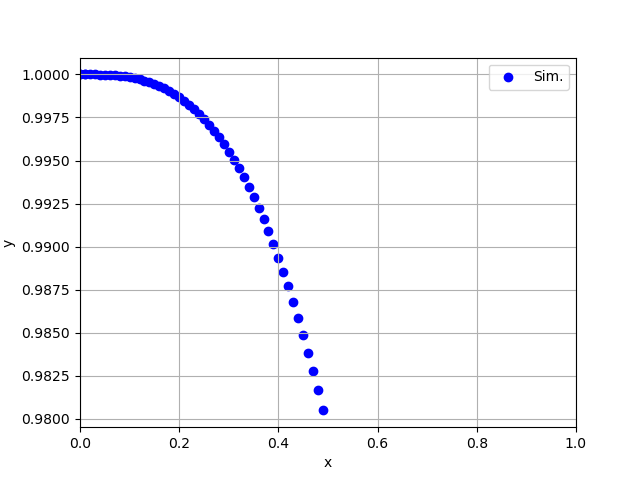
\includegraphics[width=1\columnwidth]{figs/fig.png}
				\label{stemplot}
			\end{figure}
	\end{frame}
	\end{document}
